%\documentclass{beamer}
\documentclass[mathserif,notheorems]{beamer} % option notheorems
\usepackage[utf8]{inputenc}
\usepackage{tikz-cd}
\usepackage{tikz}
\usepackage{multicol}
\usepackage{graphicx}
\usepackage{subcaption}
\usepackage{algorithm}
\usepackage[noend]{algpseudocode}
\graphicspath{{talk_images/}}
%\usetikzlibrary{graphs}
%\usetikzlibrary{graphdrawing}
%\usegdlibrary{trees}
\newcommand{\Olo}{$\mathcal{O}(\log_{2}n)$}

%%%%%%%%%%%%%%%%%%%%%%%%%%%%%%%%%%
\usepackage{amsmath, amsthm, amssymb, amsfonts}
\setbeamertemplate{theorems}[numbered] % to number

\theoremstyle{plain} % insert bellow all blocks you want in italic
\newtheorem{theorem}{Theorem}%[section] % to number according to section

\theoremstyle{definition} % insert bellow all blocks you want in normal text
\newtheorem*{definition}{}%[] % to number according to section
\newtheorem*{idea}{Proof idea} % no numbered block
%%%%%%%%%%%%%%%%%%%%%%%%%%%%%%%%%%

%%%%%%%%%%%%%%%%%%%%%%%%%%%%%%%%%%
\usetheme{Madrid}
\usecolortheme{beaver}
\setbeamertemplate{itemize items}[default]
\setbeamertemplate{enumerate items}[default]
\setbeamertemplate{section in toc}[square]

\title[ICPC Tutorial]{ICPC Tutorial}
\subtitle{Intro. to ICPC, Binary Search, DP, Graphs} 
\author[Ankesh] % (optional, for multiple authors)
{
	Ankesh Gupta
}
\institute[IIT D] % (optional)
{
  Dept. of Computer Science and Engineering\\
  Indian Institute of Technology, Delhi
} 
\date[\today] % (optional)
{}

%\logo{\includegraphics[height=1.5cm]{lion-logo.png}}

\AtBeginSection[]
{
  \begin{frame}
    \frametitle{Table of Contents}
    \tableofcontents[currentsection]
  \end{frame}
}
% \AtBeginSubsection[]
% {
%   \begin{frame}
%     \frametitle{Table of Contents}
%     \tableofcontents[
%             currentsection,
%             % currentsubsection,
%             % subsectionstyle=show/shaded/hide
%     ]
%   \end{frame}
% }

\algdef{SE}[SUBALG]{Indent}{EndIndent}{}{\algorithmicend\ }%
\algtext*{Indent}
\algtext*{EndIndent}
%%%%%%%%%%%%%%%%%%%%%%%%%%%%%%%%%

\begin{document} 
\frame{\titlepage}
\begin{frame}
\frametitle{Table of Contents}
\tableofcontents
\end{frame}

\section{ICPC}
\begin{frame}
\begin{definition}<+->[What is ICPC?]
General introduction to competition logistics
\end{definition}
\end{frame}

\section{Binary Search}
\subsection{Why?}
\begin{frame}
\frametitle{Why?}
\begin{figure}[!htb]
	\begin{subfigure}{\textwidth}
		\centering
		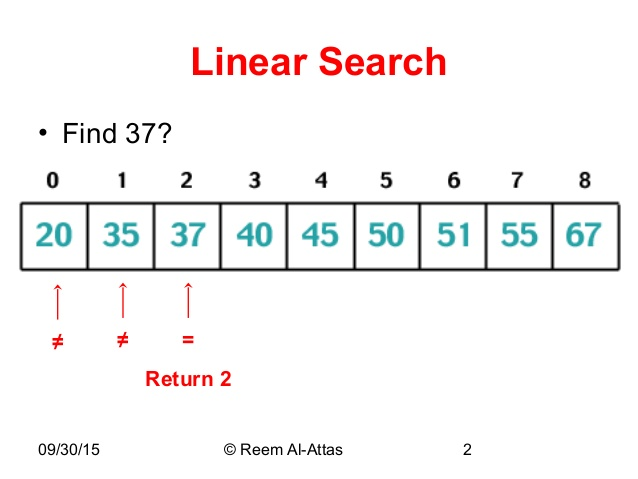
\includegraphics[width=1\textwidth]{ls.jpg}
	\end{subfigure}
\end{figure}

\end{frame}

% \section{Binary Search}
\subsection{Analysing?}
\begin{frame}
\frametitle{Analysing}
\begin{definition}<+->[Complexity]
\begin{enumerate}
	\item Complexity $\mathcal{O}(n)$
	\item Can we exploit the structure of array?
	\item Array is Partially Ordered!
\end{enumerate}
\end{definition}
\end{frame}

\subsection{Picture is worth a 1000 words!}
\begin{frame}
\frametitle{Picture is worth a 1000 words!}
\begin{figure}[!htb]
	\begin{subfigure}{\textwidth}
		\centering
		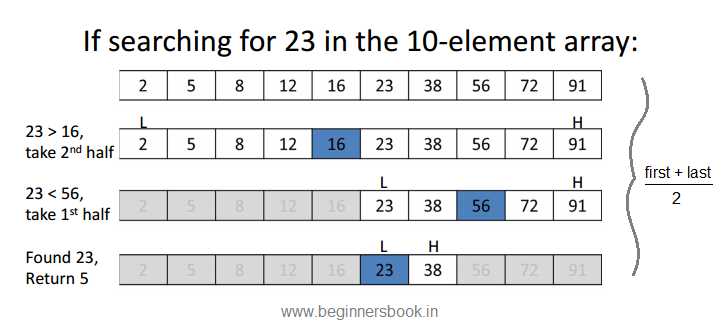
\includegraphics[width=1\textwidth]{binary-search-algorithm.png}
	\end{subfigure}
\end{figure}

\begin{definition}<+->[Complexity]
	\begin{itemize}
		\item Complexity is \Olo. Intuition how many times can a number be divided by $k$ - $\mathcal{O}(\log_{k} {n})$
	\end{itemize}
\end{definition}
\end{frame}

\subsection{Problems}
\begin{frame}
\frametitle{Problems}
	\begin{definition}[Trivial]
		\begin{itemize}
			\item Find largest element less than a given element
			\item Find smallest element greater than a given element
		\end{itemize}
	\end{definition}
	\begin{definition}[Better]
		\begin{itemize}
			\item \href{https://tex.stackexchange.com/questions/107832/how-to-create-internet-link-in-pdf}{AGGRCOW - Aggressive cows}
			\item \href{https://codeforces.com/contest/689/problem/C}{C. Mike and Chocolate Thieves}
			\item Many more - \href{https://www.hackerearth.com/practice/algorithms/searching/binary-search/practice-problems/}{Hackerearth}
			\item Advanced Concept: \href{https://www.hackerearth.com/practice/algorithms/searching/ternary-search/tutorial/}{Ternary Searches},\href{https://codeforces.com/blog/entry/45578}{Parallel Binary Searches}
		\end{itemize}
	\end{definition}
\end{frame}

\section{Dynamic Programming}
\begin{frame}
\begin{definition}[Dynamic Programming a.k.a DP]
	\begin{itemize}
		\item Brief introduction
		\item Problem discussion
		\item Ideal Tutorial: \href{https://www.topcoder.com/community/competitive-programming/tutorials/dynamic-programming-from-novice-to-advanced/}{Topcoder}
	\end{itemize}
\end{definition}
\begin{definition}[Comments]
	\begin{itemize}
		\item Advanced Topics: \href{https://codeforces.com/blog/entry/8219}{DP Optimizations}
		\item Generally easy to code, tough to spot/figure-out state
		\item Can be coupled with any algorithm you know - general technique very useful in life: \href{https://codeforces.com/blog/entry/58589\#comment-422219}{Discussion}
	\end{itemize}
\end{definition}
\end{frame}

\section{Graphs}
\begin{frame}
\begin{definition}[Graphs]
	\begin{itemize}
		\item Most beautiful! personal favourite :)
		\item Brief introduction
		\item Problem discussion
	\end{itemize}
\end{definition}
\begin{definition}[Comments]
	\begin{itemize}
		\item Very useful! Immense applications!
		\item Generally short codes and recursive thinking.
		\item Some must know trivia - Traversals, Shortest Paths Algorithms
		\item Many advanced topics: Bridges, Articulation Points, Strongly Connected Components(SCC), Heavy-Light Decomposition, Centroid Decomposition, 2-SAT and many-many more.
	\end{itemize}
\end{definition}
\end{frame}

\section{Closing Remarks}
\begin{frame}
\frametitle{Closing Remarks}
	\begin{itemize}
		\item CP is an art!
		\item Don't force it upon. Give time.
		\item Don't rush to solution/editorials. Try once more! It's thinking that matters!
		\item Make a good team.
		\item Speed matters!
		\item Everything you need is online! 
		\item Awesome community! Brilliant people!
		\item It helps knowing CP in interview. Helps arrive at efficient solutions quickly.
	\end{itemize}
\end{frame}

\begin{frame}{}
  \centering \Large
  \emph{Thank You!\\}
  \emph{Questions?}
\end{frame}
% \begin{frame}
% \begin{definition}[Thank You!]
% \end{definition}
% \begin{definition}[Any questions?]
% \end{definition}
% \end{frame}
\end{document}


